\documentclass[tikz,border=2mm]{standalone}
\usepackage[utf8]{inputenc}
\usepackage[T1]{fontenc}
\usepackage{tikz}
\usetikzlibrary{arrows.meta, positioning}
\usepackage{pgfplots}

\pgfplotsset{compat=1.18}

\begin{document}
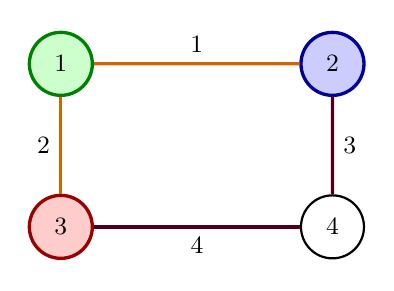
\begin{tikzpicture}[
  scale=1.15,
  every node/.style={font=\small},
  v/.style={circle, draw, thick, minimum size=8mm, inner sep=0pt},
  start/.style={v, fill=green!20, draw=green!50!black, very thick},
  exit/.style={v, fill=blue!20, draw=blue!60!black, very thick},
  rat/.style={v, fill=red!20, draw=red!60!black, very thick},
  pairA/.style={very thick, draw=orange!80!black},
  pairB/.style={very thick, draw=purple!40!black}
]

% Nodes
\node[start] (1) at (0,1.8) {1};
\node[exit]  (2) at (3,1.8) {2};
\node[rat]   (3) at (0,0)   {3};
\node[v]     (4) at (3,0)   {4};

% Edges in pair A: 1 and 2
\draw[pairA] (1) -- node[above] {1} (2);
\draw[pairA] (1) -- node[left]  {2} (3);

% Edges in pair B: 3 and 4
\draw[pairB] (2) -- node[right] {3} (4);
\draw[pairB] (4) -- node[below] {4} (3);

\end{tikzpicture}

\end{document}